% !TeX spellcheck = en_GB
% !TeX root = memoco-report.tex

\section{Exact method}
\label{chap:cplexm}
The exact algorithm makes use of the IBM CPLEX C++ APIs to solve a problem to optimality. In order to model the TSP problem a network flow model is used, as described in the assignment text. \\
The specific linear programming model used and its decision variables are presented below. The set $A$ is the set of edges of the graph, which in this case is a complete graph.
\begin{itemize}
	\item $x_{ij}$ is the amount of 'flow' passed from $i$ to $j,~\forall~(i,j)\in A$
	\item $y_{ij} = 1$ if the edge $(i,j)$ ships some flow, $0$ otherwise $\forall~(i,j)\in A$.
\end{itemize}
\begin{align}
	&\min \sum\limits_{i,j:(i,j)\in A} c_{ij}y_{ij}\\
	&~s.t.~\sum_{i:(i,k)\in A}x_{ik} - \sum_{j:(k,j)\in A, j\ne 0}x_{kj}~~~=~1~~~~~~~~~~~~~~~~~~~~~~\forall~k \in N \setminus \{0\}\label{eq:flow}\\
	&~~~~~~\sum_{j:(i,j)\in A} y_{ij}~~~~~~~~~~~~~~~~~~~~~~~~~~=~1~~~~~~~~~~~~~~~~~~~~~~\forall~i \in N \label{eq:sumi}\\
	&~~~~~~\sum_{i:(i,j)\in A} y_{ij}~~~~~~~~~~~~~~~~~~~~~~~~~~=~1~~~~~~~~~~~~~~~~~~~~~~\forall~j \in N \label{eq:sumj}\\ 
	&~~~~~~~x_{ij}~~~~~~~~~~~~~~~~~~~~~~~~~~~~~~~~~~~\le~(|N|-1)~y_{ij}~~~~~~~\forall~(i,j) \in A,j\ne 0 \label{eq:constrxy}\\
	&~~~~~~~x_{ij} \in \mathbb{R}_+~~~~~~~~~~~~~~~~~~~~~~~~~~~~~~~~~~~~~~~~~~~~~~~~~~~~~~~~\forall~(i,j) \in A,j\ne 0 \label{eq:constrx}\\
	&~~~~~~~y_{ij} \in \{0,1\}~~~~~~~~~~~~~~~~~~~~~~~~~~~~~~~~~~~~~~~~~~~~~~~~~~~~~\forall~(i,j) \in A
\end{align}

Actually, when adding the variables $x$ and $y$ to the model, variables $x_{ij}~\forall~(i,j) \in A,j\ne 0$, instead of being unbounded like in constraint \ref{eq:constrx}, they are forced to be in range $[0,N-1]$. The model is still valid, since constraint \ref{eq:constrxy} also bounds the variables in this range.

\subsection{Creation of the model}
The linear programming model is set up in the function \texttt{setupLP} in file \texttt{CPLEX.cpp}.\\
During the creation of the model, its decision variables $x_{ij}$ and $y_{ij}$ are first added one by one (for each possible value of $i$ and $j$) through the appropriate CPLEX functions to a C array. Variables with $i = j$ are not added, since no loops on the same point is allowed. Considering that this variables have to be referenced later during the definition of the constraints, their position in the CPLEX array is recorded in two bidimensional vectors, one for the $x$, called \texttt{xMap}, and one for $y$ variables, named \texttt{yMap}. In this way variable $x_{ij}$ can be later referenced easily with \texttt{xMap[i][j]} for all $i$ and $j$. After defining the variables of the problem, the constraints \ref{eq:flow} - \ref{eq:constrxy} are inserted. Constraint \ref{eq:constrxy} was reformulated as $x_{ij} - (|N|-1)y_{ij} \le 0$ because the CPLEX APIs require all the variables in the left-hand side and only constants in the right side of the equation.\\
The model can be solved calling the function \texttt{solve}, which calls the IBM CPLEX solving routines for a minimization problem. The solution can then be retrieved using the method \texttt{getSolution} which returns a \texttt{TSPsolution} object, which wraps many useful information about the final solution, and is used for both the exact method and the heuristic one.

\section{Heuristic method}
\label{chap:heuris}

The implemented heuristic is inspired by a popular local search method called Lin-Kernighan heuristic, originally proposed in 1973 in \cite{LinK73}. The algorithm can be considered a generalization of the k-opt algorithm: one of the drawbacks of this algorithm is that the parameter $k$ must be fixed in advance. Instead, the Lin-Kerighan algorithm decides at each iteration, for ascending values of $k$, whether an interchange of $k$ edges provides a better solution. Thus, the algorithm is specified in terms of exchanges that can convert one tour into another: given a feasible interchange of $k$ edges (a \textit{k-move}), the algorithm tries to determine if there exists a $k+1$-move that improves the tour further. 
During each iteration, given a feasible tour, the algorithm repeatedly performs exchanges that reduce the length of the current tour, until a tour is reached for which no exchange yields an improvement. This process may be repeated many times from initial tours generated in some possibly randomized way \cite{Helsgaun2000}.\\
So at each iteration the algorithm tries to determine the largest set $X=\{x_1, x_2, ..., x_j\}$ and $Y=\{y_1, y_2, ..., y_j\}$ such that if edges in $X$ (also called the \emph{broken} edges) are removed and replaced by $Y$ (the \emph{joined} edges) the produced tour is a feasible improved (i.e. less costly) solution. Of course, a naive brute force algorithm searching for this sets, would quickly become impractical to use, due to the exponential running time. In order to produce a reasonably efficient local search procedure, the algorithm reduce the search space using the following criteria:

\begin{enumerate}
	\item \emph{Sequential exchange criterion}: each pair of edges $(x_i, y_i)$ and $(y_i, x_{i+1})$ must share one vertex. If $t_1$ and $t_2$ are the vertices of edge $x_1$, then in general for all $i \ge 1$ exchanges are performed this way: $x_i=(t_{2i-1}, t_{2i})$ and $y_i=(t_{2i}, t_{2i+1})$ and $x_{i+1}=(t_{2i+1}, t_{2i+2})$.\\ All \emph{sequential} k-opt moves can be found by concatenating smaller sequential moves, but \emph{non sequential} moves cannot be found with this algorithm. An example of such a move is given in \cref{fig:doublebridge}.
	\item \emph{Feasibility criterion}: for every $i \ge 3$, $x_i=(t_{2i-1}, t_{2i})$ is chosen so that if $t_{2i}$ is connected to $t_1$ the resulting configuration is a tour (i.e. a feasible solution). It can be seen that at most one choice for $x_i$ satisfies this constraint, as showed in \cref{fig:feasibility-moves}. Exceptionally, when $i=2$, the originally proposed algorithm allowed for the choice of an $x_i$ which violates this rule. According to the original paper this was done to strengthen the procedure by giving the algorithm a way to recover from previous wrong choices, but allowing this kind of backtracking at every levels would significantly increase the running time;
	\item \emph{Positive gain criterion}: let $g_i=cost(x_i) - cost(y_i)$ be the gain by exchanging two edges, and let $G_i=g_1+g_2+...+g_i$ be the partial sum of the gains up to the $i^{th}$ exchange. This criterion requires that each $y_j$ is chosen in a way such that $G_j$ is positive. This choice is justified by the fact that if a sequence of numbers has a positive sum, there is a cyclic permutation of these numbers such
	that every partial sum is positive \cite{Helsgaun2000};
	\item \emph{Disjunctivity criterion}: sets $X$ and $Y$ must be disjoint. 
\end{enumerate}
In the implemented algorithm, the move size threshold which allows for the exceptional violation of the \emph{feasibility criterion} (set to $2$ in the paper), is not fixed but it can be modified in the configuration file \texttt{config.yml}. In this way the influence of this parameter on the solution quality could be tested and optimized.

\begin{figure}[h]
	\centering
	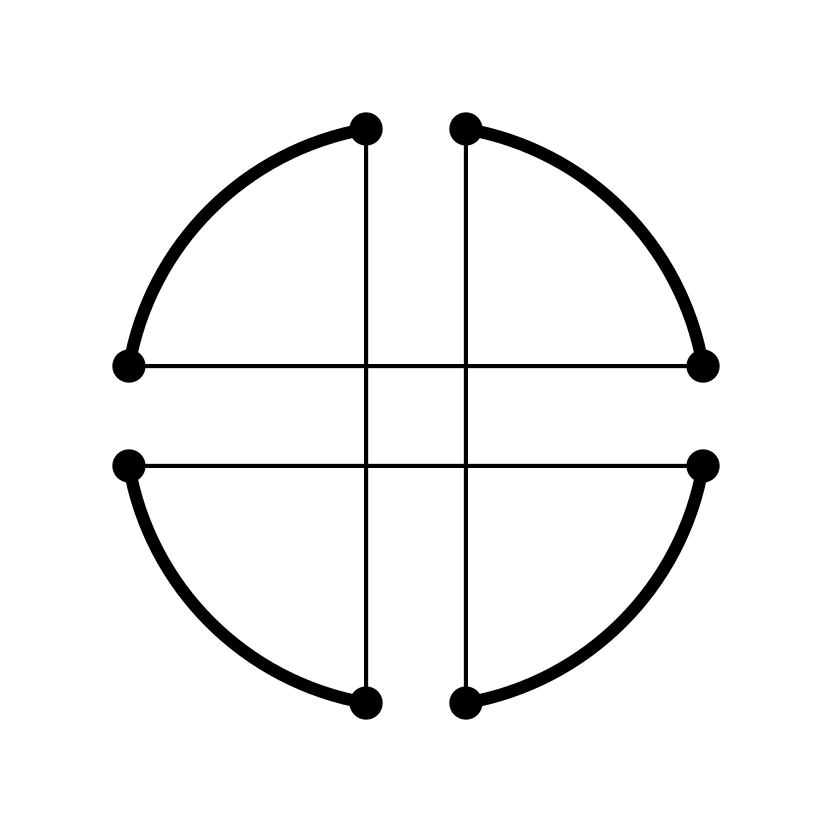
\includegraphics[width=6cm]{double-bridge}
	\caption{A non sequential \emph{double bridge} move with $k=4$}
	\label{fig:doublebridge}
\end{figure}

\begin{figure}[h]
	\centering
	\begin{subfigure}[c]{0.31\textwidth}
		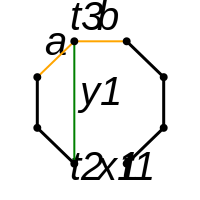
\includegraphics[width=\textwidth]{path-choices}
		\caption{The two possibles edges to break after choosing $y_1$: $a$, $b$}
	\end{subfigure}
	\begin{subfigure}[c]{0.31\textwidth}
		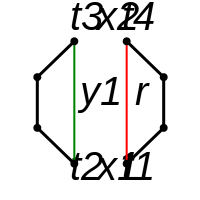
\includegraphics[width=\textwidth]{path-wrong}
		\caption{Breaking edge $b$ violates the feasibility criterion}
	\end{subfigure}
	\begin{subfigure}[c]{0.31\textwidth}
		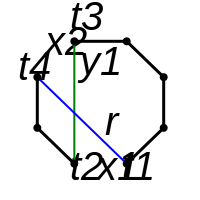
\includegraphics[width=\textwidth]{path-right}
		\caption{Breaking edge $a$ allows to close the tour correctly}
	\end{subfigure}
	\caption{Only one candidate for $x_i$ satisfies the feasibility criterion, which is enforced for $i$ greater than a fixed threshold value. In this case breaking edge $a$ is the right choice, since removing edge $b$ and relinking with edge $r=(t_4,t_1)$ would not produce a feasible tour.}
	\label{fig:feasibility-moves}
\end{figure}

\subsection{Stopping criterion}
The algorithm uses the same stopping criterion suggested in the original paper. In particular, when the algorithm finds a feasible tour with a move of size $k$, it checks whether the total gain is the best seen so far. If it is then it is the best improvement seen and it saves the current solution, and tries to improve further with a $k+1$-move. If this does not improve the solution the algorithm returns the solution it saved. On the other hand, if the size $k$ move yields a feasible tour which is not the best seen so far, the algorithm stops, since it knows there is a better move, with size smaller than $k$, that produces a better tour.\\
By accepting only improving solutions, the algorithm is guaranteed to eventually stop, since it cannot loop over the same local optima.

\subsection{Tour structure}
A tour is maintained as a vector $v$ of pairs, where $v_i$ gives a pair with the two vertices which precedes and follows $i$ in the current tour. To this purpose every vertices (point) of the instance is numbered from $0$ to $N-1$ and its number is used as index to access the tour structure. Creation of such structure takes time $O(N)$ from a list of vertices where $N$ is the problem size. This allows constant time checks and retrieval of the two edges to break. Moreover, the distance between each vertex (the cost of each edge) is kept in a $N\times N$ sized matrix.

\subsection{Neighbourhood function}
\label{ssec:neighbourhood}
In a local search algorithm the neighbourhood function describes which solutions are explored at every step. In this case every neighbour is generated with a $k$-move from the initial solution and the algorithm tries to increase $k$ at each step.\\
In the described algorithm, for a given $i$, a step consists in breaking an edge of the tour $x_i$ and replacing it with  and edge $y_i$ chosen with the criteria described in \cref{chap:heuris}. Every step generates a new neighbour.
If we fix the vertex $t_{2i-1}$ belonging to joined edge $y_{i-1}$, there are exactly two edges that can be broken. That's because the \emph{sequential exchange criterion} requires that $x_i$ must share an endpoint with $y_{i-1}$ and this endpoint is exactly $t_{2i-1}$. Additionally, by the \emph{feasibility criterion}, there is only one choice of $x_i$ that will produce a feasible tour, while breaking the other will inevitably split the graph into two connected components (as seen in \cref{fig:feasibility-moves}). \\
Starting from vertex $t_{2i-1}$ the algorithm analyses the two possibilities giving the precedence to the edge with higher cost, since is the best one to remove. Only if the feasibility criterion is violated the procedure will try to remove the other edge.\\
In order to choose an edge $y_i$, the algorithm finds all possible edges starting in $t_{2i}$ which are
\begin{itemize}
	\setlength\itemsep{0.05em}
	\item not part of the current solution;
	\item not already broken (i.e. $\notin X$);
	\item not already joined (i.e. $\notin Y$).
\end{itemize}
A simple approach would be to choose as $y_i$ the candidate edge with the lowest cost, since we want to maximize the gain. The paper suggests using a less greedy approach, by looking also at the successive edge $x_{i+1}$. This has the additional benefit of avoiding useless search, as would happen by joining a promising candidate only to find out, when selecting the next edge to break, that no such operation is possible (for example because the only alternative has already been broken). \\
Thus for each candidate edge to join, the possible $x_{i+1}$ are analysed, and the potential gain of adding $y_i$ and removing $x_{i+1}$ is computed. Since the algorithm does not know which choice of $x_{i+1}$ gives the feasible tour, if neither choice can be discarded because of other reasons (e.g. already broken, intensification constraints), both choices are considered and the potential gain is the average of the two gains. So the potential gain is the average gain to expect by joining $y_i$ and breaking $x_{i+1}$. Ideally, the neighbourhood function should predict which candidate $x_{i+1}$ is the actual feasible choice that the algorithm will eventually make. Unfortunately, checking this for every possible candidate is quite costly for instances with considerable size, since checking if a sequence of edges represent a feasible tour takes time $O(N)$ on average, and the number of candidates grows linearly with $N$ too.\\
Instead of using the average potential gain to rank the candidates for joining, two alternative approaches using the worst gain and the best possible gain has been tested. Calibration tests on an instance of 90 points determined that this approach produced slightly better results than the others.

%\begin{enumerate}
%	\item Start from a (possibly random) feasible solution;
%	\item Choose an initial vertex $s$;
%	\item Remove an edge $x_1 = (s, v)$ which belongs to the current solution and add an edge $y_1 = (v, z)$ ($z \ne s$) which does not belong to the current solution, such that the gain of this move (removal and insertion) is positive;
%	\item Perform step 3 with the following additional constraints:
%	\begin{itemize}
%		\item the edge to remove ($x_i$) must share 1 vertex with the previous added edge ($y_{i-1}$);
%		\item the edge to remove $x_i = (a, b)$ must be chosen such that if $b$ reconnects to the starting vertex $s$ with edge $(b, s)$, the produced solution is feasible;
%		\item the gain (decrease of objective value) of the solution found with previous constraint must be greater than the best increase found so far.
%	\end{itemize}
%	If the second and third conditions are satisfied, the procedure saves this feasible solution, updates the best gain, and proceeds to step 5. Otherwise it tries the other possibility for $x_i$. If this fails too the procedure stops, and the last saved solution is returned;
%	\item Repeat step 4. When no improving solution can be found set the current best solution as starting solution and restart from step 2.
%\end{enumerate}

\subsection{Enhancements}
This basic algorithm scheme can be enhanced in many ways. The next sections describe some additional strategies implemented in this project.

\subsubsection{Search intensification}
\label{sssec:intensification}
Between the iterations the algorithm may find some 'good' edges which belongs to the optimal solution or to some reasonably good ones. Subsequently some time may be lost by repeatedly breaking and adding them, while not exploring some more profitable moves. \\
In addition these 'good' edges are likely to be present in many of the best solutions (local optima) found between iterations. In order to direct the search towards more promising solutions, the algorithm keeps track of the edges shared by best $S$ solutions by computing their intersection.\\ 
On the other hand, if the top-S solutions do not include the global optimum, this approach  may prevent the algorithm from breaking some edges which do not belong to the optimum, thus preventing the algorithm from finding it.\\ To mitigate this problem, the intensification procedure is applied only after a specified number of improving moves (i.e. after a fixed $i$). This means that the algorithm has a way to escape this additional constraint for a small number of moves, allowing it to recover from previous sub-optimal choices.\\ 
Additionally, after a local optima is found, the objective value is tested to see if it is better than one of the top-S solutions and in this case the worst solution is replaced with the new one and the intersection is updated.\\
A max-heap data structure is used in order to efficiently replace the worst (i.e. with higher objective value) local optima, and the collection of edges of each tour is maintained in a \texttt{std::set} ordered container, which allows the intersection procedure to take time $O(N\cdot S)$ where $N$ is the number of edges in a feasible tour.\\
Instead of considering just the top-S solutions to do the intersection, the original paper proposed to keep the intersection of all tours from the beginning. During some early tests this seemed to worsen the results with respect to the runs without intensification, so this change was made, and a small reduction of running time has been registered, since the algorithm excludes some choices from its neighbourhood.
In choosing the parameter $S$ it is important to keep in mind that intensification is done only after $S$ local optima are found, so one should ensure that this number is suitable for the problem dimension, since a very large number with a small problem would probably be ineffective.

\subsubsection{Avoiding duplicate solutions}
\label{sssec:checkout}
The authors of the algorithm stated that 30\% to 50\% of running time could be saved by keeping track of previous local optima and stopping the algorithm if the current local optima is the same seen before. This is justified by the fact that if the algorithm couldn't improve this solution before, it's unlikely it can do it now. While this sounds reasonable, in the proposed implementation no particular speed-up was registered. In part, this may be due to different computing capabilities, considering that the algorithm was devised in 1973.\\
Since trying to improve a previously found local optima will likely fail, the proposed algorithm adopts a slightly different strategy in this eventuality: instead of stopping, it restarts from a different starting edge and proceeds normally until it finds a different solution, or it determines no better tour exists. While this does not guarantee an improvement in running time, it makes the algorithm redirect the search in a different direction, which is probably more useful that exploring the neighbourhood of a previous solution.\\
To do this, an \texttt{std::set} data structure is used, which maintains a sorted collection (ordered by tour cost) of all the feasible tours found at each iteration. This container guarantees logarithmic insertion and search operations.\\
As a possible improvement to this strategy, one could keep track of the edges modified while converging to the previously encountered solution, and make sure that at least some of these are not added again, which can potentially lead to the same solution again, or to a very similar one.

\clearpage
\subsection{Random restart}
The described heuristic is run from a randomized initial solution, like the one in \cref{fig:randomtour}. This simple strategy allows the algorithm to escape local optima and differentiate the provided solutions. Using an initial solution generated with a fast constructive heuristic has been tried, and a faster convergence has been registered, even though the produced solution was often not better than the solution generated from a random initial solution.
Despite this, the starting tour has a significant impact on the heuristic performance, since it determines the edges that will be tried for the first move. Indeed the algorithm often does not explore more than the first two-three candidates to be joined. This explains why the initial tour greatly contributes to the final result.\\
By restarting the heuristic many times on the same instances of the synthetic dataset of size $> 90$, on average, the heuristic will produce tours 0.5\% from the optimal one, but the best solution found during a reasonable number of restarts is usually much closer to the optimal one. This strategy has been implemented in the file \texttt{utilities.cpp}, where the procedure \texttt{runILK} is defined for this purpose. Setting the desired number of restarts in the \texttt{config.yml} configuration file (parameter \texttt{LK\_iterations}) will restart the algorithm the specified number of times, and the final result will be the best solution found.

\begin{figure}[h]
	\centering
	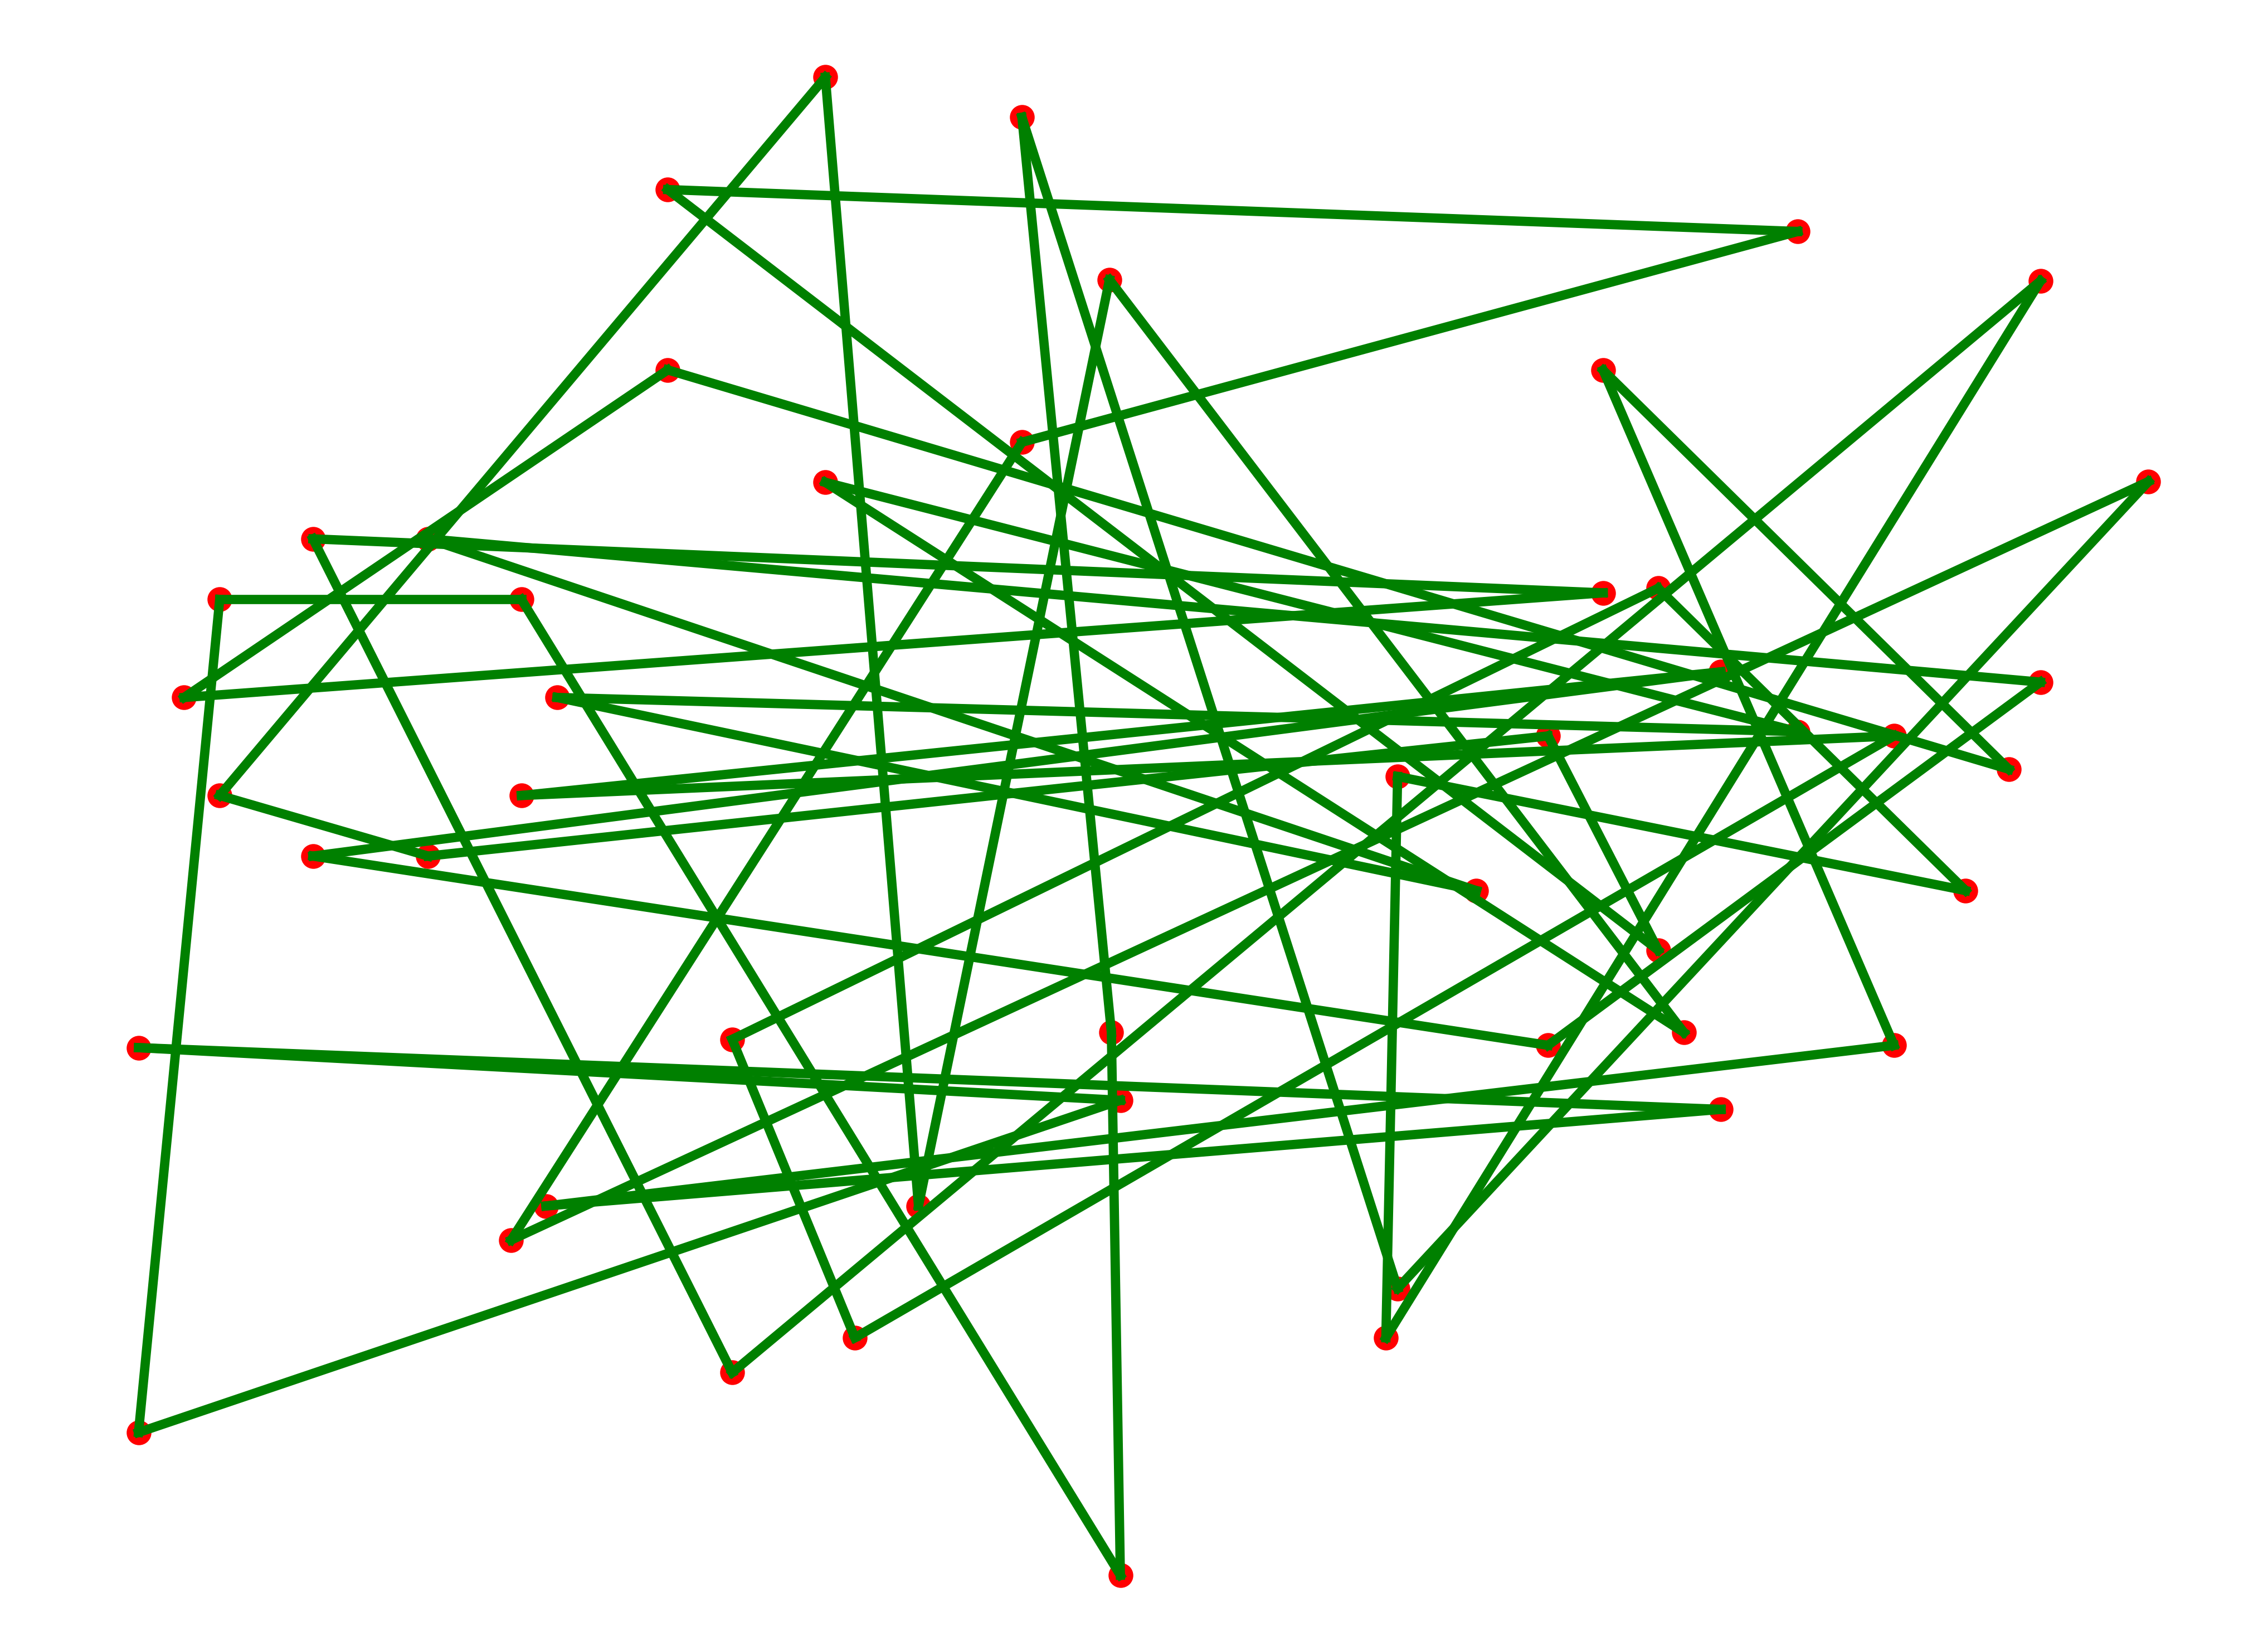
\includegraphics[width=12cm]{path_50_random}
	\caption{Random initial path on a problem with 50 points}
	\label{fig:randomtour}
\end{figure}

\clearpage
\subsection{Parameters}
\label{ssec:hyperpar}
Table \ref{tab:hyperparameters} includes a description of each parameter to be set in file \texttt{config.yml} before starting the heuristic. Calibration of this parameters are discussed in the next section.

\LTXtable{\linewidth}{parameters}

This heuristic may require some tuning to be usable with bigger problems, since some parameters can significantly increase the running time. To determine the next move, the heuristic considers at most \texttt{max\_neighbours} candidates for joining, and it may do up to \texttt{K} moves per iteration, so the worst case complexity of a single search for the best possible move is $O(max\_neighbours^K)$. This process may be repeated for up to \texttt{I} iterations. Using random restarts this entire procedure is repeated exactly \texttt{LK\_iterations} times. High \texttt{back\-track\-ing\_threshold} values allow the algorithm to violate the feasibility criterion and try more moves, but will also require more time. Low values, like 3 or 4, worked well during testing, even though 2 is more likely the best parameter for instances of size greater than 300.\\
If the algorithm spend too much searching for a move (i.e. searching for an exchange), the \texttt{K} parameter should be lowered. On the other hand, if the algorithm tends to do too many iterations, this number may be limited by lowering \texttt{I}. Reducing \texttt{K} and increasing \texttt{I} allow the algorithm to do a bigger number of smaller improvements. On the other hand increasing \texttt{K} and reducing \texttt{I} will allow for a lower number of better improvements.

\subsubsection{Calibration}
Some parameters in \cref{tab:hyperparameters} may affect the running time and the solution quality. In order to determine how much this parameters influenced this metrics and to select the best ones for the final tests, some trials were done on two different instances, one of size 90 and one of size 198 taken from TSPLIB\footnote{\url{http://elib.zib.de/pub/mp-testdata/tsp/tsplib/tsplib.html}}. Given some sets of parameters to try, every possible combination has been tested by restarting the heuristic 10 times on each combination. The results are reported in tables and discussed in the next paragraphs. Listed information includes the average percentage error, whether the optimal solution was found, the average number of iterations and the total time required for the 10 iterations. The final score is obtained by iterating the heuristic 10 times on the same instance and takes into account the average percentage relative error (w.r.t. the optimal solution computed using the exact algorithm), called $ARE$ and the total execution time for the 10 iterations, called $TT$. The score is given by \cref{eq:score}.
\begin{equation}
	\text{Score} = \cfrac{1}{1 + (ARE * TT)}
	\label{eq:score}
\end{equation}
These results were obtained by using all the features described before, and by compiling with \texttt{-O3} optimization flag. Both tests were done with \texttt{K = 100}.\\
The calibration procedure is implemented in file \texttt{calibrate.cpp}, and more tests can be done by editing the file and running the script with commands~\texttt{make calibrate \&\& ./bin/calibrate}.

\paragraph{Syntetic instance of size 90}\mbox{}\\
Table \ref{tab:calibration} reports the results of the calibration procedure on an instance with 90 points.
Other tests, which are not reported here, were run using the other two ranking strategies to sort the candidates to be joined, discussed in \cref{ssec:neighbourhood}. Strategies using the best and average gain performed similarly, while the strategy sorting by worst gain performed poorly. Three different calibrations for all three strategies has been run and the average gain strategy was selected because it reached the optimal solution more frequently then the best gain one.\\
As can e seen in \cref{tab:calibration}, considering more neighbours during the selection of the edge to join (5 instead of 2) results in a lower average error and higher running time. Additionally with value set to 5 the optimal value was found in all cases but one.\\
Additional tests were done with \texttt{backtracking\_depth} set to 2 and 3. Lowering this parameter reduce running time and also the frequency of finding the optimum, so in the table only the runs with depth 4 or 5 are listed.\\

\LTXtable{\linewidth}{calibration}

\paragraph{TSPLIB d198}\mbox{}\\
In order to select some good parameters for a non trivial instance, and additional calibration was done on a drilling problem with 198 points from TSPLIB, called "d198".\\
Since the instance is bigger, tests were done with higher values for \texttt{max\_neighbours}, \texttt{back\-track\-ing\_depth} up to 4 (5 is too much for big instances), and the number of tours used for intensification has been limited to 20 or 50. Table \ref{tab:calibration198} shows the results. This time the score is much lower because of the higher running time, so it has been multiplied by 100, to make it more readable.

\clearpage
\LTXtable{\linewidth}{calibration198}

No execution arrived at the optimal solution, but the original paper suggests that with more restarts better solutions can be found. In three runs with \texttt{max\_neighbours = 5}, \texttt{back\-track\-ing\_depth = 3} the best error of the 10 iterations was below 1.0, in particular 0.374, 0.773 and 0.425 with \texttt{intensification\_depth} to 5, 8 and 10 respectively. In the first case the average error was 4.911, which is the best one reported in the table (in bold). In this case the final score strongly penalises the executions with higher backtracking depth because of the long execution time, but the average error tends to decrease with \texttt{max\_neighbours = 5} and \texttt{back\-track\-ing\_depth = 3}.
